\documentclass[conference]{IEEEtran}
\usepackage{mathtools}
\usepackage{color}
\usepackage{listings}
\usepackage{courier}

\lstdefinelanguage{Scala}{}
\lstset{language=Scala, basicstyle={\small\ttfamily}}

% For commenting
%\newcommand{\comment}[1]{{\small \color{red} {#1}} \normalcolor}
% Use this line for leaving out comments
\newcommand{\comment}[1]{}

% Use this line to anonymize
\newcommand{\anonymize}[1]{\emph{Withheld to retain anonymity.}}
% Use this line to de-anonymize
%\newcommand{\anonymize}[1]{#1}

% Todo
%\newcommand{\todo}[1]{{\small \bf \color{red} {#1}} \normalcolor}
% Use this line to leave out
\newcommand{\todo}[1]{}

% Hide
%\newcommand{\hide}[1]{#1}
% Use this line to leave out
\newcommand{\hide}[1]{}

% Some shorthand
\newcommand{\fig}[1]{Fig.\ \ref{#1}}
\newcommand{\eq}[1]{Eq.\ \ref{#1}}
\newcommand{\sn}[1]{Sec.\ \ref{#1}}
\newcommand{\inquotes}[1]{``#1''}

% Notation commands (change all by changing here)
% Defina a capital Rho
\newcommand{\Rho}{\mathrm{P}}
% Concept relation
\newcommand{\rn}[1]{\rho_{#1}}
% Concept L1 norm
\newcommand{\rns}[1]{|\rn{#1}|_1}
% Concept relation threshold
\newcommand{\mrn}[1]{\tau_{#1}}
% Discarded concept relation sum
\newcommand{\drns}[1]{|\check{\rho}_{#1}|_1}
% Kept concept relation sum
\newcommand{\krns}[1]{|\hat{\rho}_{#1}|_1}
% Concept relation vector
\newcommand{\rv}{\Rho}
% AND concept
\newcommand{\acpt}{c_{\wedge}}
% OR concept
\newcommand{\ocpt}{c_{\vee}}
% Concept similarity
\newcommand{\sy}[1]{\sigma_{#1}}
% Approximate concept similarity
\newcommand{\asy}[1]{\tilde{\sigma}_{#1}}
% L1 norm of difference
\newcommand{\nm}[1]{L_1(#1)}
\newcommand{\dnm}[2]{|\rn{#1}-\rn{#2}|_1}
% Approximate L_1 norm
\newcommand{\anm}[1]{\tilde{L}_1(#1)}

\newcommand{\argmax}{\operatornamewithlimits{argmax}}

% Correct bad hyphenation here
\hyphenation{}

\begin{document}

\title{Hierarchical Concept Mining at Scale}

\author{\hide{
\IEEEauthorblockN{Olof G\"{o}rnerup}
\IEEEauthorblockA{Swedish Institute of\\
Computer Science (SICS)\\
SE-164 29 Kista, Sweden\\
Email: olof@sics.se}	
\and
\IEEEauthorblockN{Daniel Gillblad}
\IEEEauthorblockA{Swedish Institute of\\
Computer Science (SICS)\\
SE-164 29 Kista, Sweden\\
Email: dgi@sics.se}
\and
\IEEEauthorblockN{Theodore Vasiloudis}
\IEEEauthorblockA{Swedish Institute of\\
Computer Science (SICS)\\
SE-164 29 Kista, Sweden\\
Email: tvas@sics.se}
}}

\maketitle

\begin{abstract}
Conceptualization is often key for efficient processing and accurate understanding of data. 
We present a method that allows us to discover multiple abstraction levels in data solely using correlations between data
constituents. The method iteratively discovers higher-order concepts by representing concepts and correlations
as a graph that is transformed to a similarity graph in which higher-order concepts are mined. 
The method is scalable and can be applied on very large datasets. It is also domain-agnostic, and
can therefore be employed in a broad range of areas. No information about the internal specifics of data constituents is required 
since the method only operates on observed correlations. The method is demonstrated to capture abstraction 
levels of artists in playlist data, and of words in a corpus, and to significantly outperform state-of-the-art community 
detection algorithms used for the same purpose.
\end{abstract}

\section{Introduction}
\label{sec:introduction}

Being able to abstract data is many times necessary for tractable storage and processing, and for gaining
understanding of data and generating processes.
Although conceptualization is staple in machine learning and other fields, most current approaches
are either highly specialized for a task or domain (e.g.\ ontology learning \cite{Wong2012ontology}), 
requires extensive manual tuning or design (e.g.\ deep neural networks \cite{LeCun15}), 
are not scalable (e.g.\ agglomerative clustering \cite{Sibson73}),
or only discovers a single or a handful of abstraction levels (e.g.\ community detection \cite{Fortunato10}).

In this paper we present a general principle and method for hierarchical concept mining that is both broadly applicable, scalable, and requires
little, if any, manual tuning. The method is based on contextual correlation discovery \cite{Gornerup15}, that in turn is based on a few simple, yet powerful, principles:
Firstly, the context of an object (a person, word, molecule etc.) is its correlations to other objects (social links, co-occurrences, interactions etc.).
Secondly, similar objects have similar contexts -- they play similar roles in the data and are exchangeable. 
Thirdly, groups of inter-similar objects form an abstraction -- a concept.

Since an object can also be a concept, concepts may form higher-order concepts. Our method discovers these by
iteratively calculating correlations, transforming them to similarities, discovering new concepts, calculating their correlations and so forth. This results in 
a concept hierarchy that captures multiple intrinsic abstraction levels in the data.

\section{Related work}
\label{sec:relatedwork}

Due to the generality and fundamental nature of conceptualization, it is applied in a wide range of areas, from models 
of learning in cognitive science \cite{tenenbaum00} to coarse-graining in computational biology \cite{Saunders13}. 

One field where conceptualization is particularly explicit, however, is 
ontology learning \cite{Wong2012ontology}, which is applicable, e.g.\ in knowledge representation by providing data-driven 
hierarchical relations of data, such as automatically generated thesauri \cite{Yijun97}. A related area, that also borders topic modeling 
\cite{Blei12}, is topical hierarchy construction, 
where clustering typically is used to construct topic trees \cite{Liu12, Wang13, Wang15}. These approaches
are applied specifically on textual data using specific object relations, though, and therefore lack the generality of the method presented here.

Another related area in natural language processing is word clustering, with applications in word sense induction and disambiguation.
Different meanings of words or groups of words are then mined from data, as in the early work by Brown et al.\ \cite{Brown1992} 
and Lin\ \cite{Lin1998}, and related approaches by Pantel et al.\ \cite{Pantel02} and de Cruys et al.\ \cite{Cruys11}. 
In comparison to our approach, these methods do either not scale to very large datasets, or generalize
words in at most two abstraction levels, whereas our method can comfortably generate hierarchies of arbitrary depth using huge datasets.

Word clustering is typically based on Harris' distributional hypothesis that words are characterized by the contexts in which they occur in language \cite{Harris54}.
This has also been the basis for many word embedding methods, such as GloVe \cite{Pennington2014} and word2vec \cite{Mikolov-2013},
 that learn word features and represent these in relatively low dimensional vector spaces. A generalization of the same hypothesis is used in our method, 
 specifically in the correlation to similarity transformation, but it is in our case not limited to natural language. 

In deep learning, stacked layers in neural networks are used to learn features at different abstraction levels \cite{LeCun15, Hinton06}. 
While these approaches have been used with great success in several applications, 
such as machine translation \cite{Jean15} and topic classification \cite{Bordes14}, 
deep learning has the drawbacks that it requires considerable tuning and, as a black box, lacks interpretability. 
In contrast, the method presented here has few parameters and is completely transparent.

We represent concepts and correlations as a graph that we transform to a similarity graph in which we mine higher-order concepts.
The latter step is akin to community detection, for which there is an abundance of algorithms; see \cite{Fortunato2010} for a review.
Note though that we re-calculate correlations and similarities of newly discovered concepts at each iteration. 
This way we successively build \inquotes{native} correlation and similarity graphs with vertices constituting higher-order concepts. 
Furthermore, with respect to the current abstraction level, concepts are grouped at a fine resolution at each iteration. This allows us 
to capture higher-order concepts across scales without the resolution limit that constrains many community detection algorithms \cite{Fortunato07}.

\section{Methods}
\label{sec:methods}

\subsection{Preliminaries}
\label{sec:preliminaries}
We begin by specifying terminology used in this paper.
Let $C = \{i\}_{i=1}^n$ be a set of \emph{objects}, where each object has a correlation, $\rn{i,j}$, 
to each other object. The \emph{context} of an object $i$ is its 
vector of correlations to every other object, $\rn{i} = (\rn{i,j})_{j=1}^n$. Under the assumption that an object is 
characterized by its context, the similarity between two objects $i$ and 
$j$, $\sy{i,j}  \in [0, 1]$, is defined as the relative $L_1$-norm of the difference between their respective contexts, $\rn{i}$ and $\rn{j}$
\cite{Gornerup15}:
\begin{equation}\label{eq:sim}
\sy{i,j} = 1 - \frac{\dnm{i}{j}}{\rns{i} + \rns{j}}.
\end{equation}
In the \emph{correlation graph} of $C$ with respect to $\rn{i,j}$, denoted $\mathcal{R}_{\rn{}} = (C, R)$, 
vertices constitute objects and  edges $r_{i,j} \in R$ have weights $\rn{i,j}$. The \emph{similarity graph} of $C$ with 
regard to $\rn{i,j}$, $\mathcal{S}_{\rn{}} = (C, S)$, is the undirected graph where weights of edges $s_{i,j} \in S$ are 
given by $\sy{i,j}$. 

A \emph{concept} is a set of objects that have relatively high inter-similarities
in comparison to similarities to other objects. A concept can also be an object, 
and a \emph{hierarchical} (or \emph{higher-order}) concept is a concept that consists of other concepts.
A \emph{primitive} object is an object that is not a concept.

\subsection{Mining hierarchical concepts}
\label{subsec:conceptmining}

Our method takes as input a set of primitive objects and a correlation function and outputs a set of 
higher-order concepts. This is achieved by iteratively transforming a correlation graph to a similarity graph, 
merging similar concepts and then replacing their constituents in the correlation graph. 

There are many ways to specify a merging criterion, and here we use one of the simplest possible: two concepts $i$ and $j$
are merged if they have an edge $(i, j)$ that has the highest weight both for $i$ and $j$. That is, $i$ and $j$ are merged if
\begin{equation}\label{eq:mergecriterion}
(i, \argmax_k \sy{i,k}) = (\argmax_k \sy{k, j}, j).
\end{equation}
We call this criterion \emph{Mutual max}. 

The algorithm is specified as follows:
\begin{enumerate}
\item Input objects $C$ and a correlation function $\rn{}$.
\item \label{start} Build a correlation graph $\mathcal{R}_{\rn{}}$.
\item Transform $\mathcal{R}_{\rn{}}$ to a similarity graph $\mathcal{S}_{\rn{}}$.
\item Extract $\mathcal{H} = \{(i, j)\}$ where $(i, j)$ fulfills \eq{eq:mergecriterion}.
\item Replace $i$ and $j$ with $(i, j)$ in $C$ for all $(i, j) \in \mathcal{H}$.
\item If $ \mathcal{H} \neq \emptyset$ repeat from \ref{start}.
\item Output $C$.
\end{enumerate}

This approach is related to standard agglomerative clustering \cite{Sibson73}, but there are some key differences: 
Since we update the correlation graph at each iteration according to $\rn{i,j}$, we express correlations between 
concepts natively rather than indirectly through linkages. Importantly, our approach also enables us to merge 
concepts \emph{in parallell}, which makes the method scalable in a cluster setting.

\subsection{Implementation}
\label{subsec:implementation}

\begin{figure*}
\begin{lstlisting}
1: val pairs = edges.map{case (i, j, w) => (i, (j, w))}.
2:                   reduceByKey((a, b) => if(a._2 > b._2) a else b).
3:                   map{case (i, (j, w)) => (if(i < j) (i, j) else (j, i), 1)}.
4:                   reduceByKey(_ + _).filter{case ((i, j), s) => s == 2}.keys()
\end{lstlisting}
\caption{Scala code for extracting Mutual max pairs using Apache Spark. Input: an RDD (resilient distributed dataset) \texttt{edges} 
with dual directed edges $(i,j,w)$ and $(j,i,w)$. 1: create key-value pairs from vertices to weighted edges. 2: For each vertex, 
find the edge with the largest weight. 3: Sort max edges by vertex ids and replace weights with counts. 4: Count edges 
(i.e vertex pairs), extract those that occur twice and discard counts.}
\label{fig:code}
\end{figure*}

The method is implemented in Scala and uses the in-memory cluster computing framework Apache Spark \cite{Zaharia-2012}.
To enable transparency and reproducibility, the source code is available in an online 
repository.\footnote{\anonymize{https://github.com/sics-dna/hierarchical-concepts}} All datasets used in this paper are also
freely available.

In our experiments (cf.\ \sn{sec:setup}) the correlation function is defined in terms of concept co-occurrence counts, $\kappa_{i,j}$
(note, however, that our method is applicable for any concept correlation function).
These are in turn given by \emph{configuration} counts, $\lambda_{\tau}$ for configuration $\tau$.  
By configuration we mean an observation in data, such as a set of objects in a sliding window (or an ngram) 
in a sequence of objects.\footnote{\emph{Context} would have been a better term, but we omit to use it here to avoid confusion 
with the contexts in the correlation graph.} 
We begin by counting all configurations, and then create key-value pairs, $\Lambda$, where configuration ids and their counts are keyed by
the objects that occur in those configurations. For example, 
$\Lambda = ((a, (\tau, \lambda_{\tau}), (b, (\tau, \lambda_{\tau}), (c, (\tau, \lambda_{\tau}))$ for objects $a,b,c \in \tau$. 
This results in redundancies, but enables fast co-occurrence counting by self-joining $\Lambda$ followed 
by a reduction transformation to sum up the counts. 

The co-occurrence counts are then mapped to correlations using some measure $\rn{}$
(conditional probability, pointwise mutual information, normalized pointwise mutual information, Jaccard similarity or something else),
and we have a correlation graph. This graph is transformed to a similarity graph by the algorithm described in \cite{Gornerup15}. 
Mutual max pairs are then extracted through two consecutive map and reduce operations, followed by a filter operation as described in \fig{fig:code}.
The keys of the elements in $\Lambda$ keyed by $i$ and $j$ are replaced by mutual max pair $(i, j)$ through an outer join operation,
and the procedure, starting from mapping counts to correlations, is repeated.

\section{Evaluation}
\label{sec:evaluation}

\subsection{Methodology}
\label{sec:methodology}

In the quantitative evaluation our aim is to demonstrate that the hierarchical concepts output by our method
indeed capture different abstraction levels in data. To do this we adopt an approach commonly used 
in agglomerative clustering, where a hierarchy is characterized by cutting its dendrogram (genealogy of merges)
at different levels, such that leaves are partitioned into subsets with shared roots at the cut. Each level is then
characterized by its respective partition. 

In our case, a level is defined in terms of tree height (the longest path from the root to a leaf) rather than
distance as in agglomerative clustering: at level $h$, we partition primitive objects into subsets given by
objects that share a root in a subtree with height at most $h$. 

For a given concept $c$, we then compare the partition at each level $h$, denoted $\pi_h$, with a set of reference partitions 
$\omega_i$ that each represents an abstraction level. The agreement between $\pi_h$  and $\omega_i$ is quantified by the 
 Adjusted Rand index, $T(\pi_h, \omega_i)$, a standard partition similarity measure \cite{Hubert1985}. 
 Since $\pi_h$ represents a specific granularity level in the concept hierarchy, 
 we expect $T(\pi_h, \omega_i)$ to be maximized for a given $h$:
\begin{equation}\label{eq:maxrand}
\hat{T}(c, \omega_i) =  \max_j \ T(\pi_j, \omega_i).
\end{equation}
We use this value to quantify how well the hierarchy captures $\omega_i$. $\hat{T}(c, \omega_i)$ is then 
compared with the performance of three popular community detection algorithms that are applied on the similarity graph of the
primitive objects. Two of them, Infomap \cite{Rosvall2008} and Label propagation \cite{Raghavan2007}, 
produce single groupings, whereas the third one, Louvain \cite{Blondel2008}, performs hierarchical clustering.
Since the Louvain algorithm finds multiple levels of communities, we will include all levels in our comparisons (denoted 
Louvain 1, Louvain 2 etc.). Infomap and Louvain are among the best performing community detection algorithms 
available \cite{Lancichinetti09}, whereas Label propagation is included for its excellent scaling properties.

\subsection{Artists}

In our first study we build hierarchical artist concepts based on how they appear in playlists. For this purpose we use 
a dataset provided by Chen et al. \cite{Chen2012}. It consists of playlists and tag data crawled from the music 
sites Yes.com and Last.fm and represents approximately 1.7M track plays. 

We relate artists by play adjacency, so the configuration $\tau$ is an unordered pair of artists
with count $\lambda_{\tau}$ in the playlist dataset. The correlation between two concepts is given by
the pointwise mutual information \cite{Church90}:
\begin{equation}\label{eq:pwmi}
\rn{i,j} = \log_2 \frac{p_{i,j}}{p_i\ p_j},
\end{equation}
where $p_i$ and $p_j$ are frequencies of $i$ and $j$ in the playlists, 
and $p_{i,j}$ is the estimated probability that they are observed together in a configuration.

Each song is associated with a set of tags contributed by users, and we aggregate these per artist.
The tags are then used to generate reference groupings $\omega_i$ of artists at different resolution level.
We do this by associating each artist with a \emph{tag set}, which is the set of the $n$
most common tags for an artist. Artists that have identical tag sets are then grouped in $\omega_n$.
By varying $n$ we can change the granularity of these groupings. For $n=1$, there are mostly 
large groups with generic tag sets such as \{pop\}, \{rock\}, \{hip-hop\} etc, but as $n$ increases, the groups
become more niched, e.g.\ with tag sets \{rock, classic rock\} and \{rock, alternative\}.

\subsection{Words}

In our second case study we build word concept hierarchies based on their usage in text. The configuration $\tau$
is again given by unordered pairs of adjacent words, and the correlation between 
two concepts is given by their pointwise mutual information. 
Adjacency counts are collected from a Wikipedia dump from March 2015,\footnote{https://dumps.wikimedia.org/}
where we keep all alphabetic words. This results in about 3.6 billion tokens. 

To generate reference groupings of words at different resolution levels we employ WordNet \cite{Miller1995}, 
a human-made lexical database. There, words are grouped into synonym sets (synsets),
where a word may be a member of several synsets due to polysemy. To achieve a partition, we 
associate a word with the synset of its most common meaning. Grouping words that belong to the same
synsets then constitute $\omega_0$, a reference partition at the finest resolution. 
WordNet also contains hypernym relations (generalizations), that we use to generate coarser
groupings. A word is then associated with the most common hypernym of its synset, and
we group words with respect to these hypernyms. The procedure is iterated to group
words that share higher-order hypernyms, constituting $\omega_i$ for order $i$. 

\section{Experiments}
\label{sec:experiments}

\subsection{Experimental setup}
\label{sec:setup}

In the artist experiments we use the \emph{yes\_big} version of the dataset provided by 
Chen et al.\footnote{http://www.cs.cornell.edu/\~{}shuochen/lme/data\_page.html} 
Despite its name, the dataset is relatively small and therefore noisy compared to the Wikipedia corpus 
(three orders of magnitude smaller). For this reason we use the 500 most frequent
artists (out of about 2000) as primitive objects. Chen et al.\ have collected the 250 most frequent tags, from which we 
manually remove tags that are unrelated to artist genres, such as \emph{favorites}, \emph{awesome}, \emph{amazing} etc.

In the word case, we filter out the low-information stop words used by Stanford CoreNLP.\footnote{https://github.com/stanfordnlp/CoreNLP}
Of the remaining ones, primitive words are constituted by the 10000 most frequent words. To reduce low count-noise, 
very infrequent configurations (less than $10^{-7}$) are discarded. Version 3.0 of WordNet is used to generate
reference partitions.

In all experiments, an indegree threshold of 100 edges is used when doing the correlation to similarity graph 
transformations, cf.\ \cite{Gornerup15}. Increasing this threshold has little effect on the results presented here.

\subsection{Qualitative evaluation}
\label{sec:qualitative}

\begin{figure*}
\begin{center}
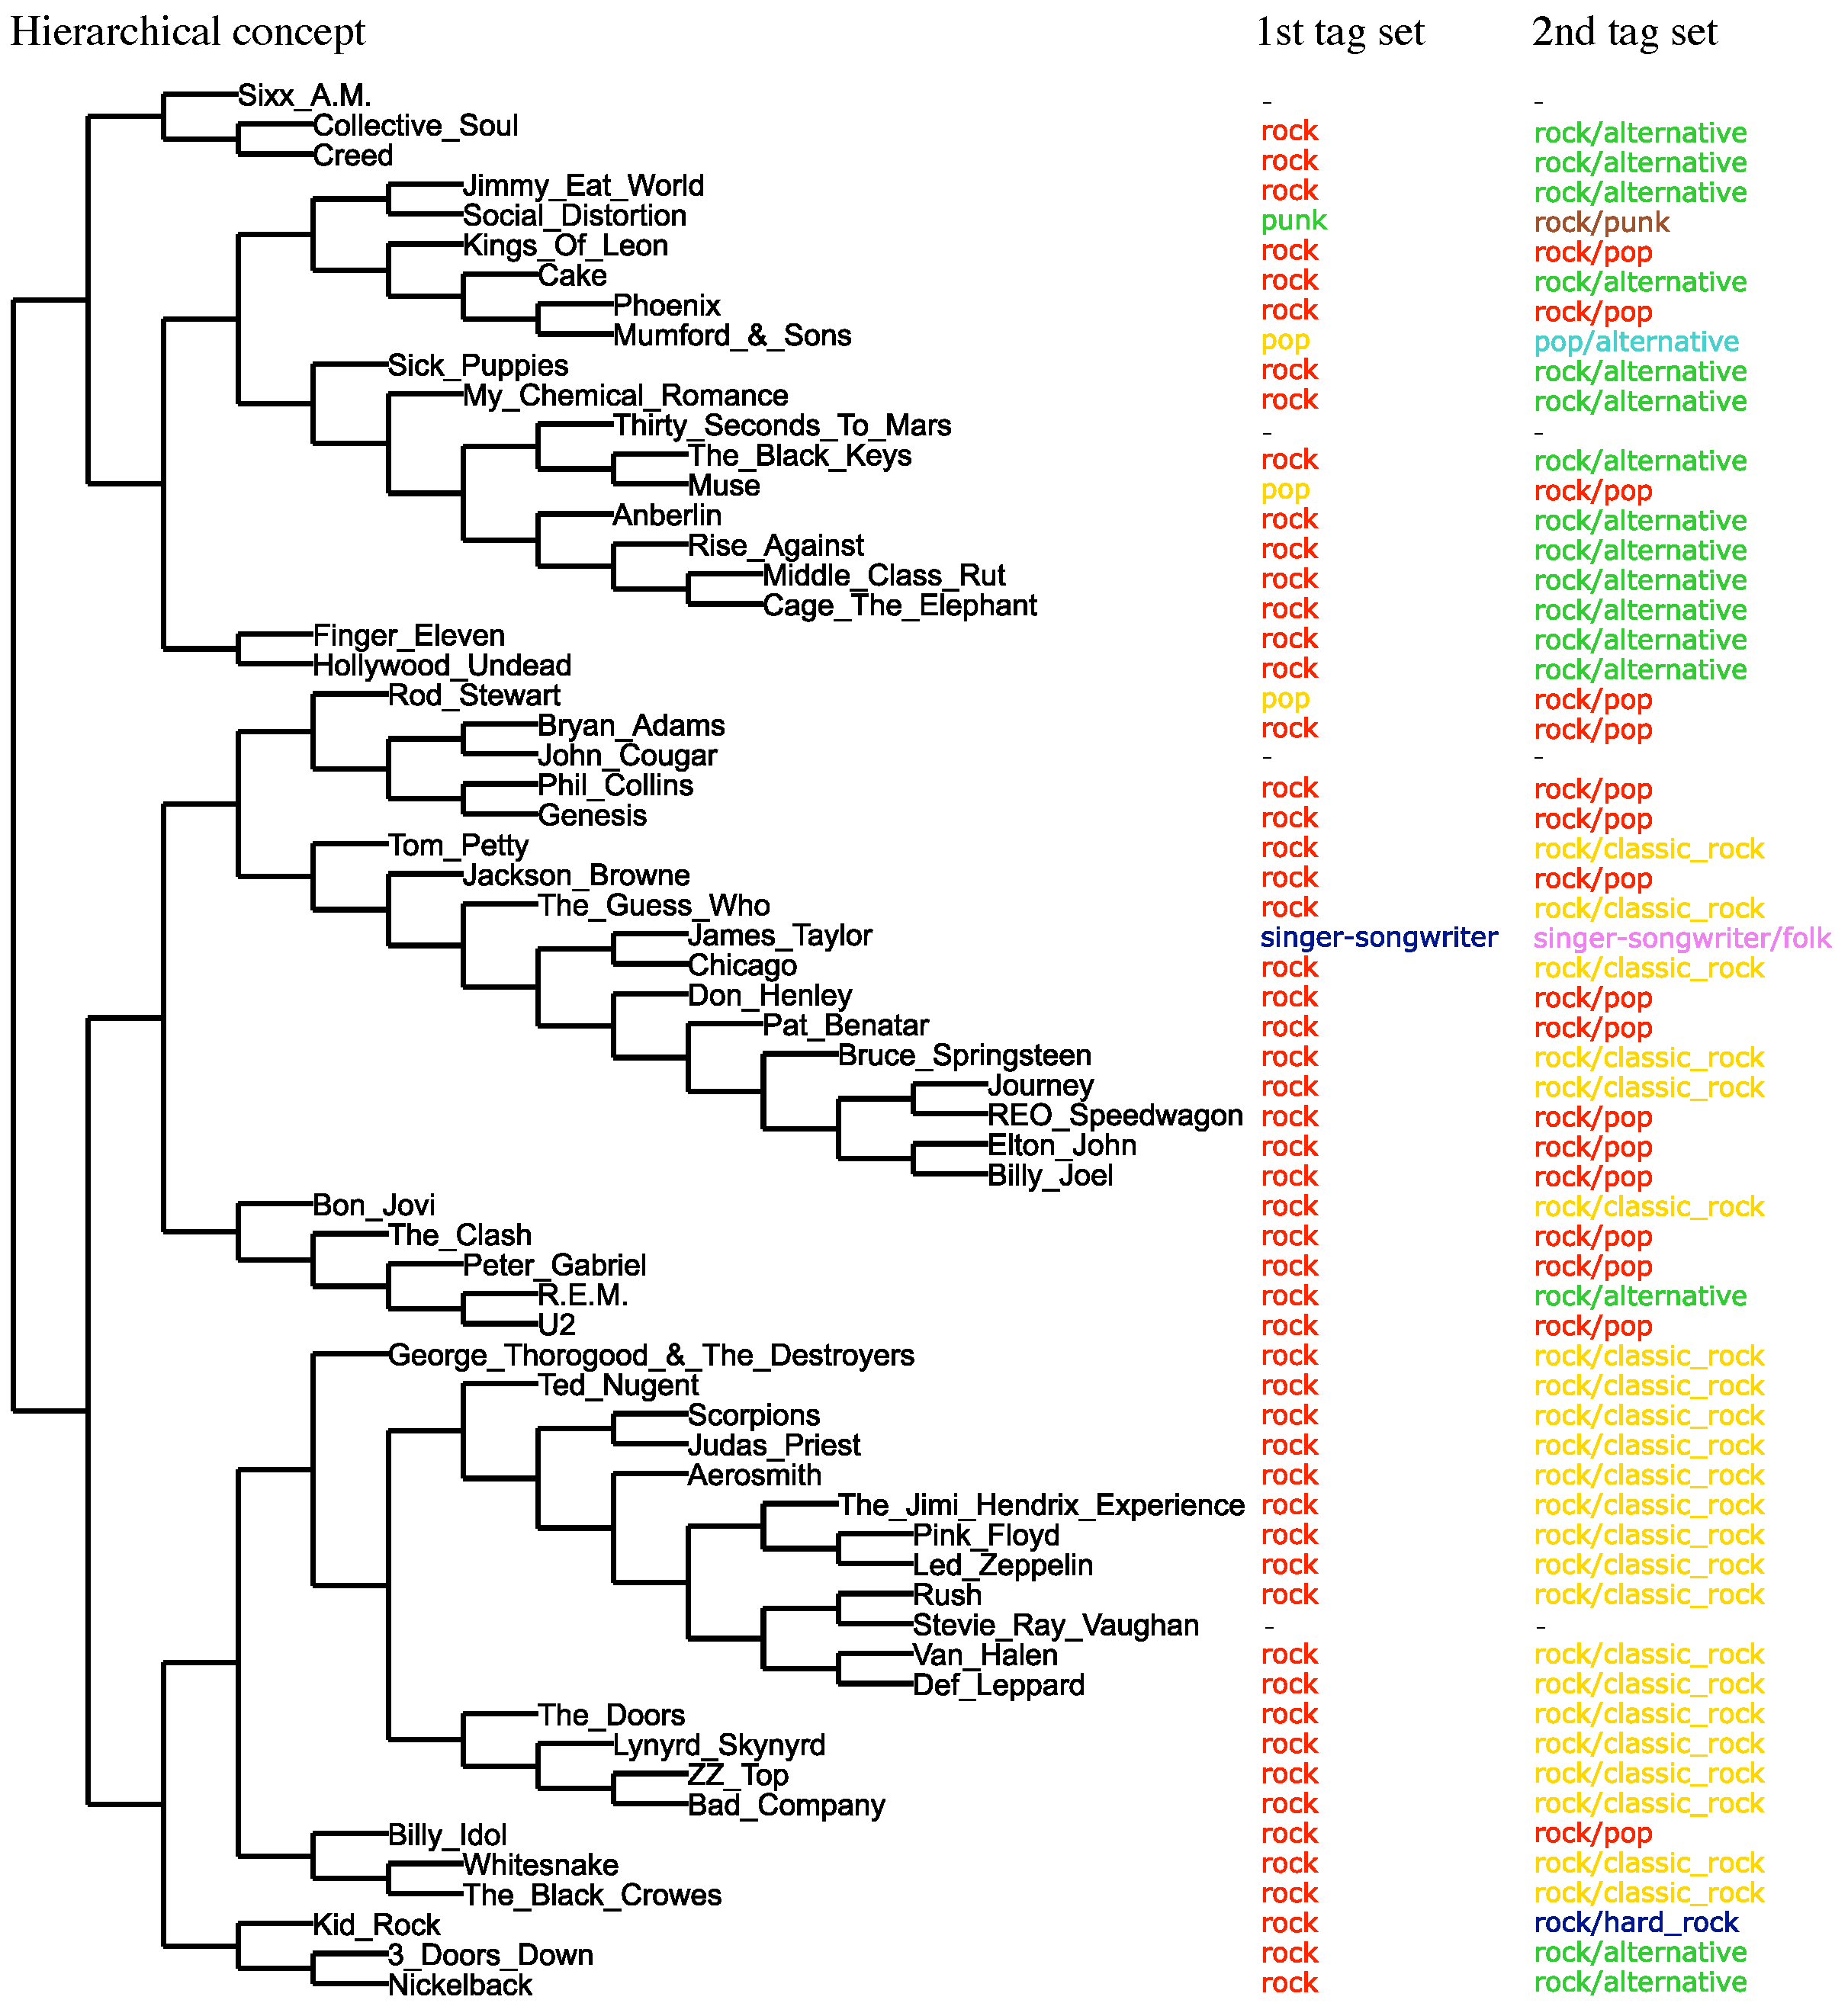
\includegraphics[width=1.55\columnwidth]{figures/artist-hierarchy-example.pdf}
\end{center}
\caption{Example of hierarchical artist concept. Missing tag sets are denoted by \inquotes{-}. The visualization was done with ETE \cite{HuertaCepas16}.}
\label{fig:artisttree}
\end{figure*}

\begin{figure*}
\begin{center}
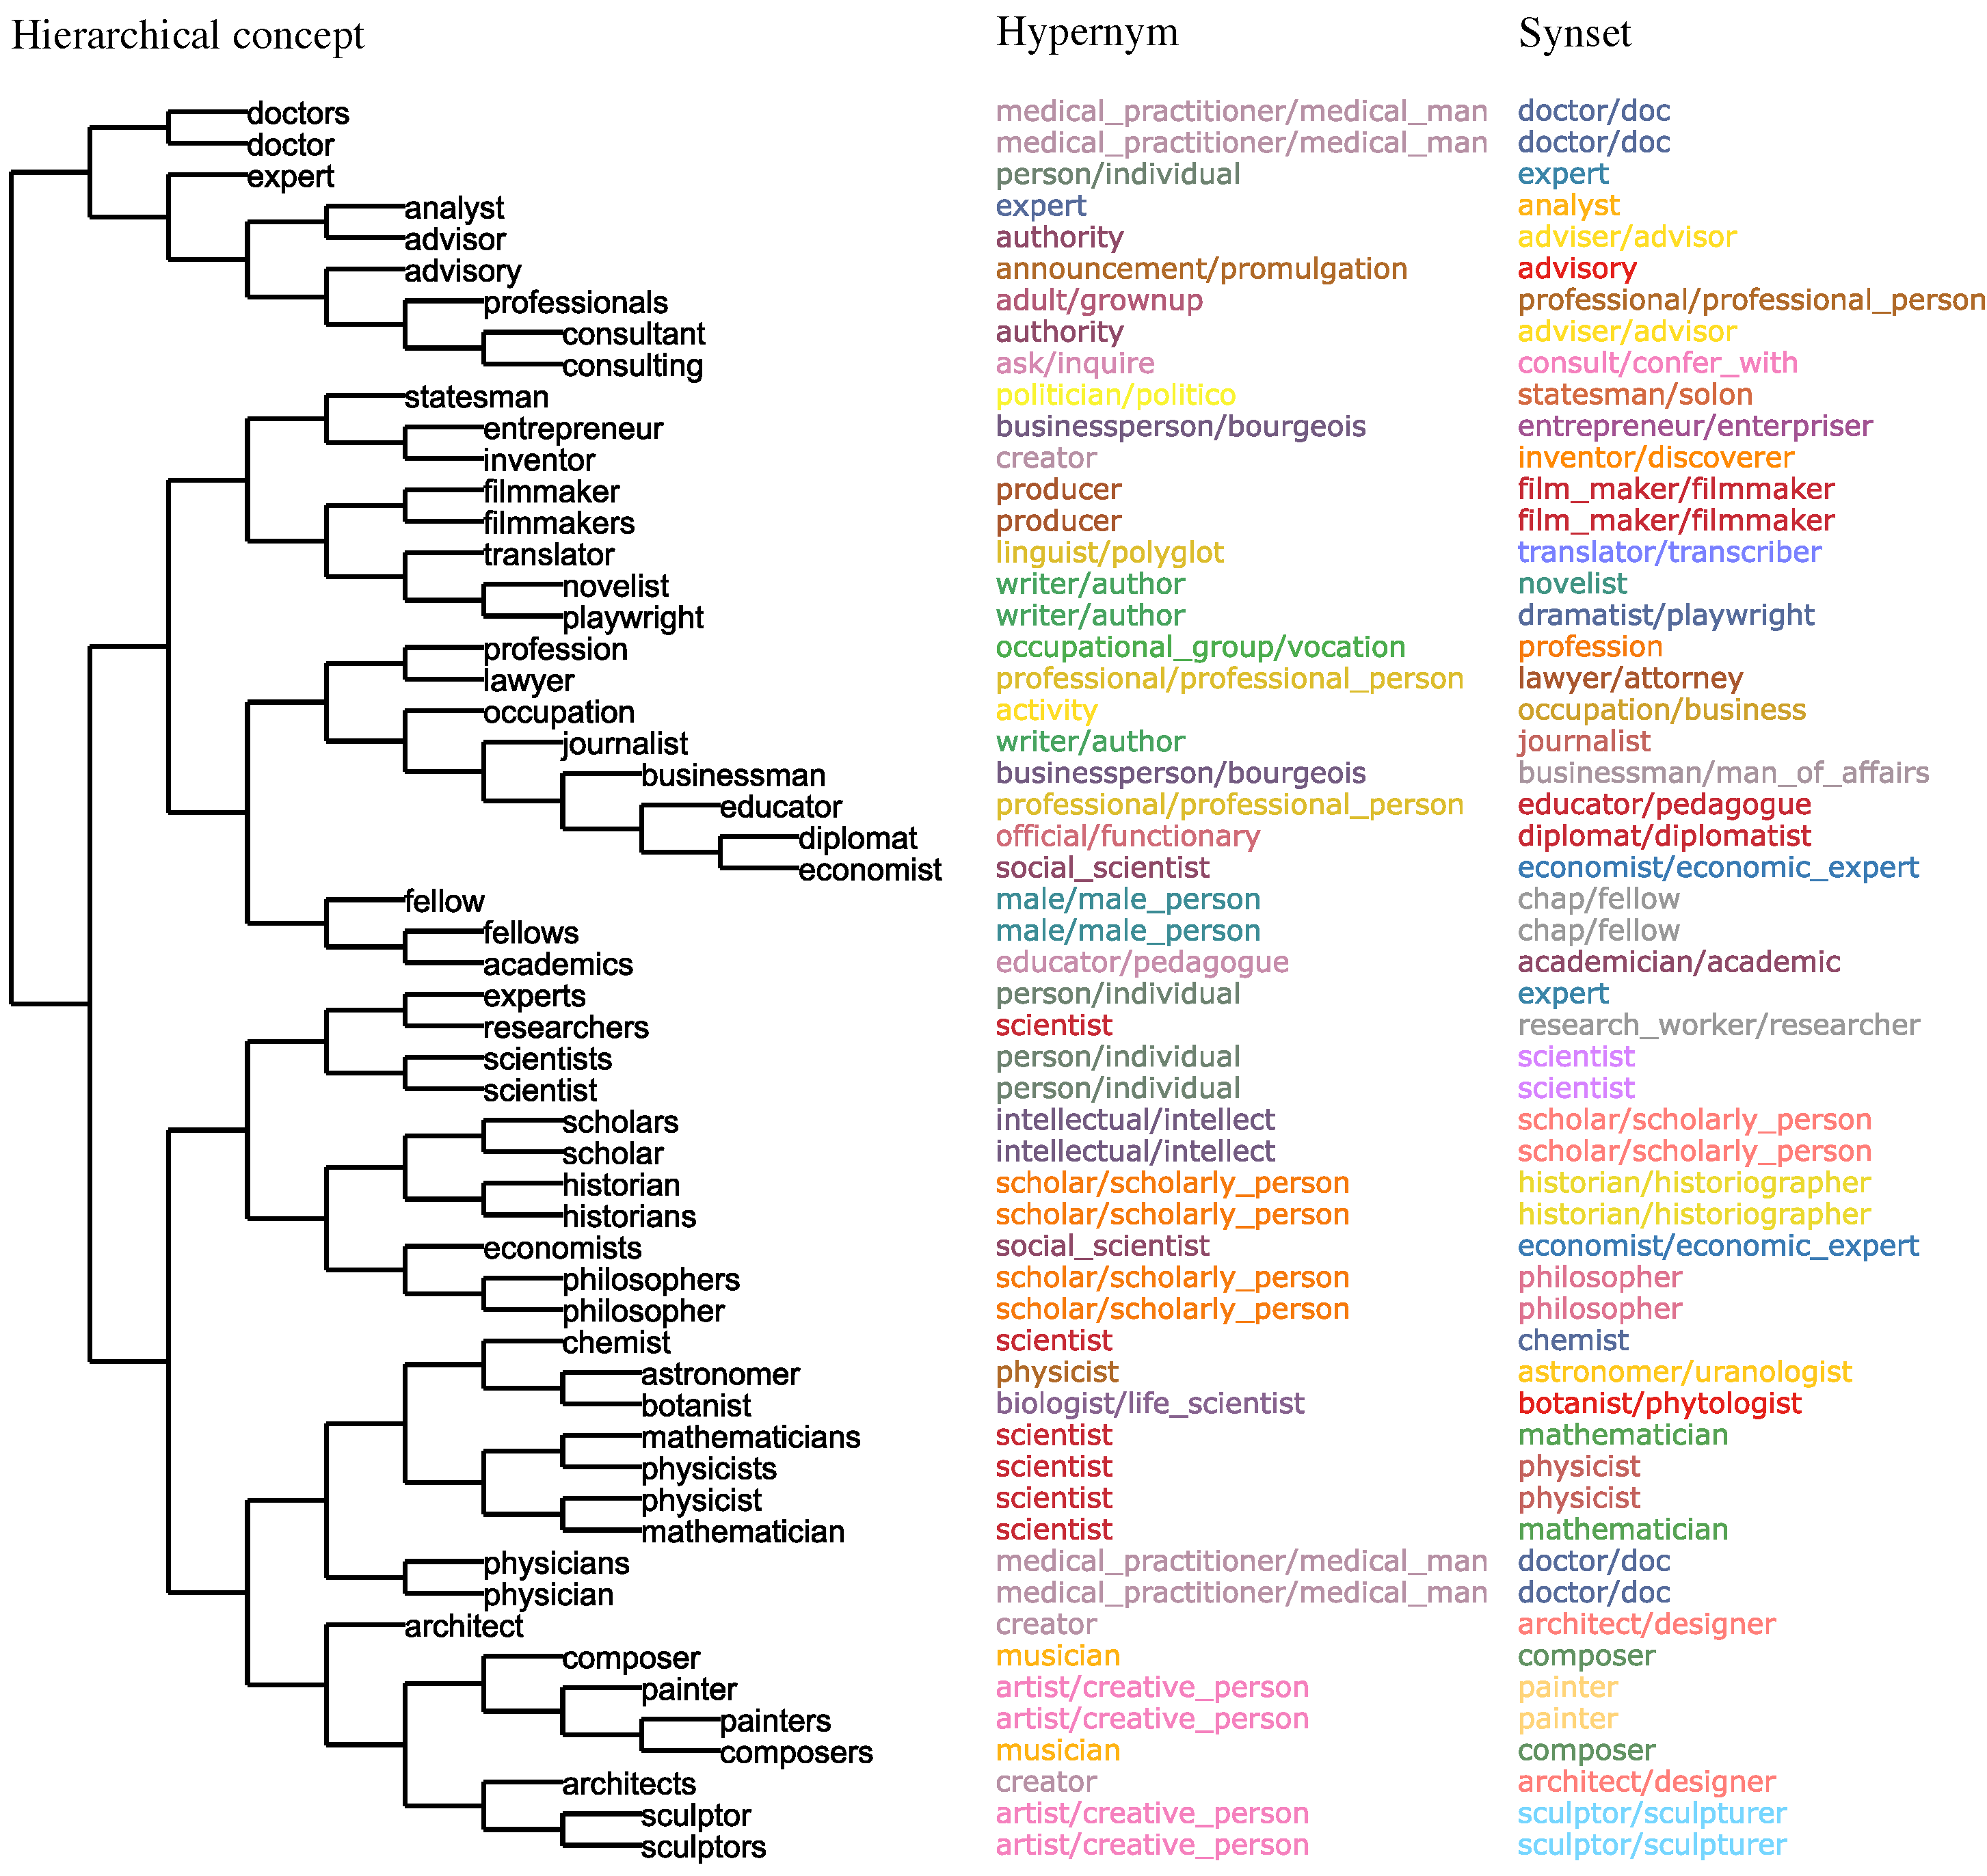
\includegraphics[width=1.7\columnwidth]{figures/word-hierarchy-example.pdf}
\end{center}
\caption{Example hierarchical word concept. The visualization was done with ETE \cite{HuertaCepas16}.}
\label{fig:wordtree}
\end{figure*}

To gain intuition about resulting hierarchical concepts, we begin by showing two example hierarchies along 
reference partitions $\omega_i$. Note that the examples represent sub-hierarchies that are parts of other, higher-order,
hierarchies (these are not possible to display due to space and resolution constraints).

In both cases it is clear that our method is able to group analogous and related concepts. This also appears to 
be true at multiple levels: For artists, see \fig{fig:artisttree}, the concept represented by the whole tree is consistent -- with a few exceptions --
with the coarse \{rock\} tag set. And as we subdivide the tree into its main branches, these reflect finer categories
given by tag sets of size 2, where \{rock, alternative\} mainly appears in one branch, \{rock, pop\} in another,
and \{rock, classic rock\} in a third. Note also that there is a slight overlap of tag sets in the two latter branches, 
which is consistent with that they form a subtree not including the \{rock, alternative\} branch.

For the word concept shown in \fig{fig:wordtree}, that predominantly represents professions, our method has also grouped related sub-concepts
on multiple levels, e.g.\ corresponding to scientists, artists, and scholars. The agreement with the WordNet categories is not
as clear as in the artist case, though, which is partly due to the much finer resolution of synsets. Note that the coarsening of the reference partition
from synsets to hypernyms is consistent with the hierarchy generated by our method, where \emph{painter} and \emph{sculptor},
for instance, are replaced by \emph{artist} in one branch, and \emph{historian} and \emph{philosopher} are merged into \emph{scholar} in another branch.

\subsection{Quantitative evaluation}
\label{sec:quantitative}

\begin{figure}
\begin{center}
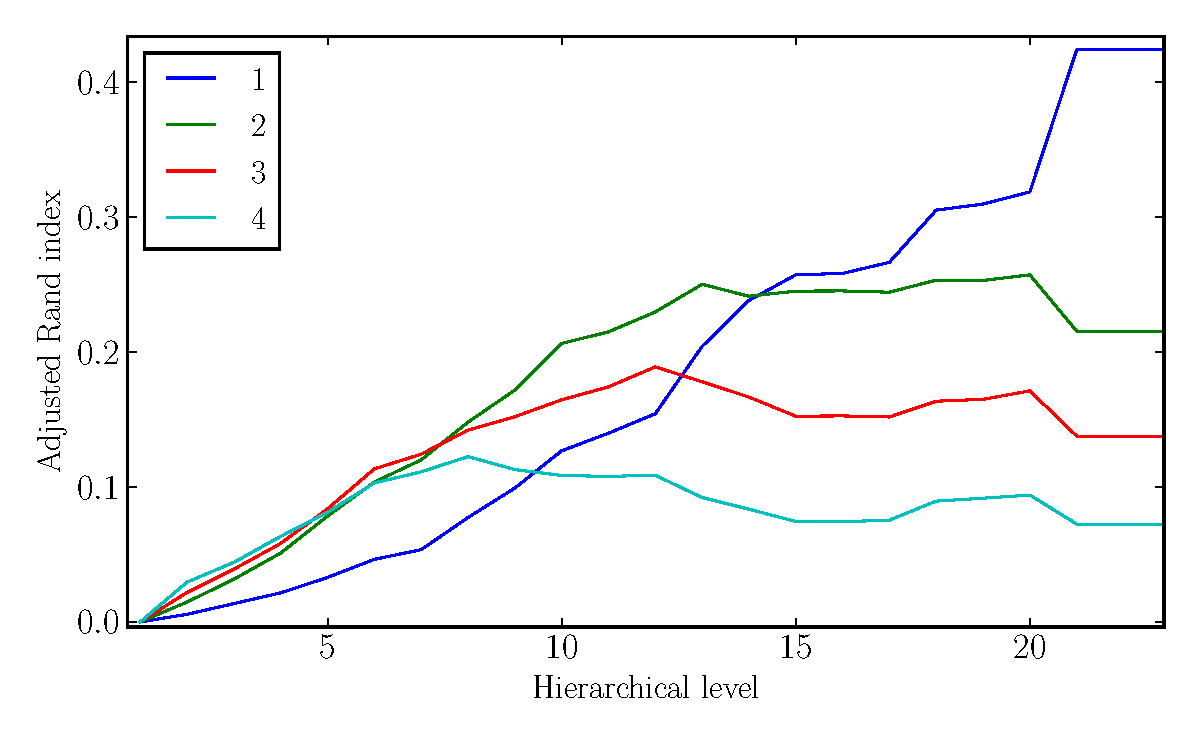
\includegraphics[width=0.9\columnwidth]{figures/1465824758-all-tags-1.pdf}
\centerline{\footnotesize{(a)}}
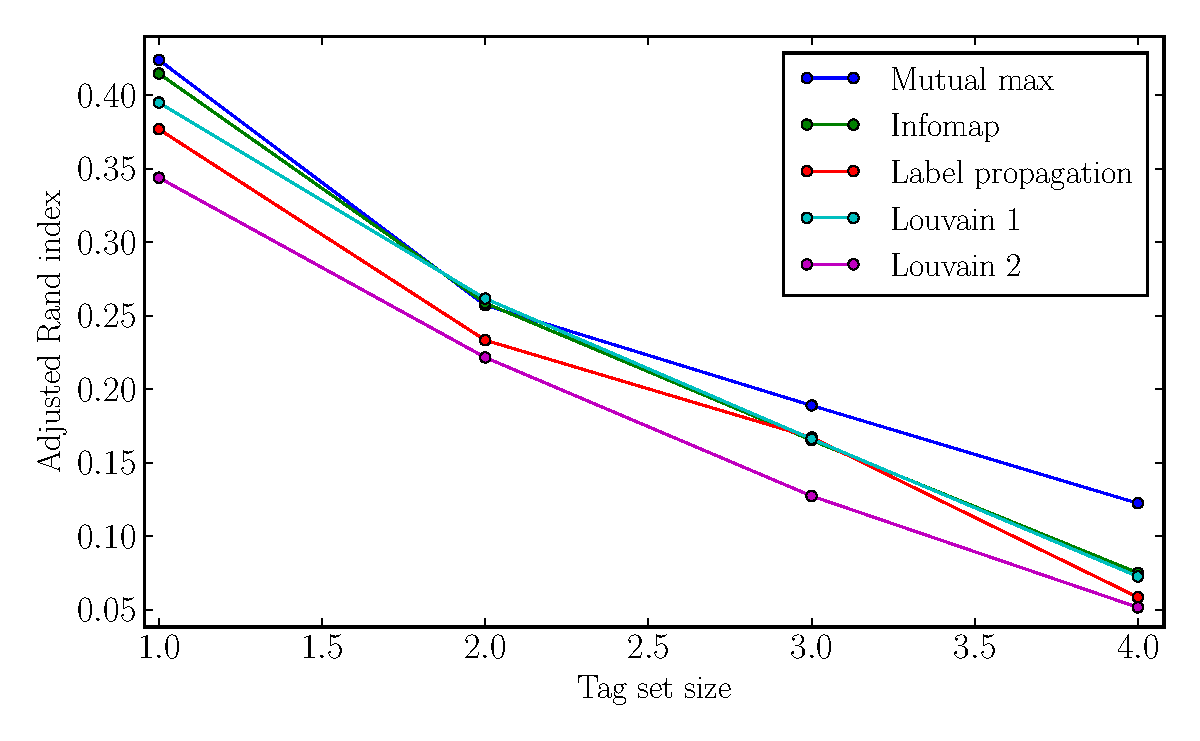
\includegraphics[width=0.9\columnwidth]{figures/1465824758-all-tags-2.pdf}
\centerline{\footnotesize{(b)}}
\end{center}
\caption{(a) Partition agreement at different levels in the artist concept hierarchy with reference partitions for tag set sizes $i$.
(b) Comparison of agreements with reference partitions for artists.}
\label{fig:artistplots}
\end{figure}

\begin{figure}
\begin{center}
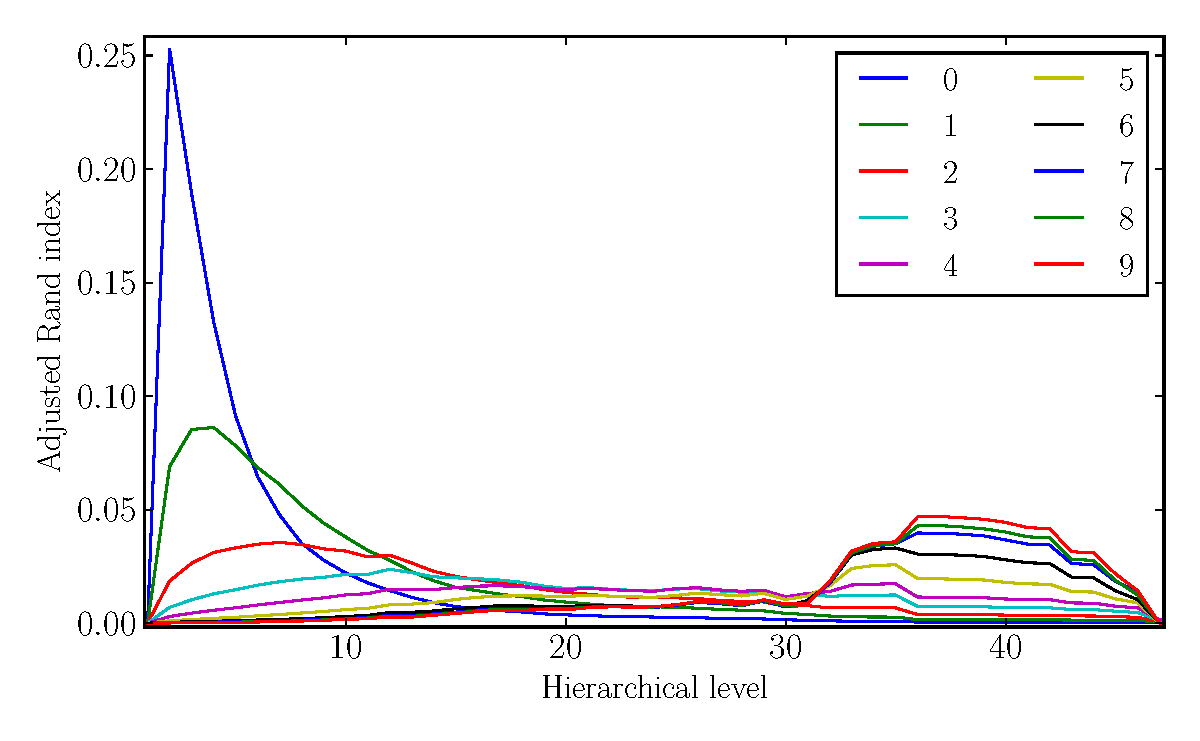
\includegraphics[width=0.9\columnwidth]{figures/1465671278-1465711376-1.pdf}
\centerline{\footnotesize{(a)}}
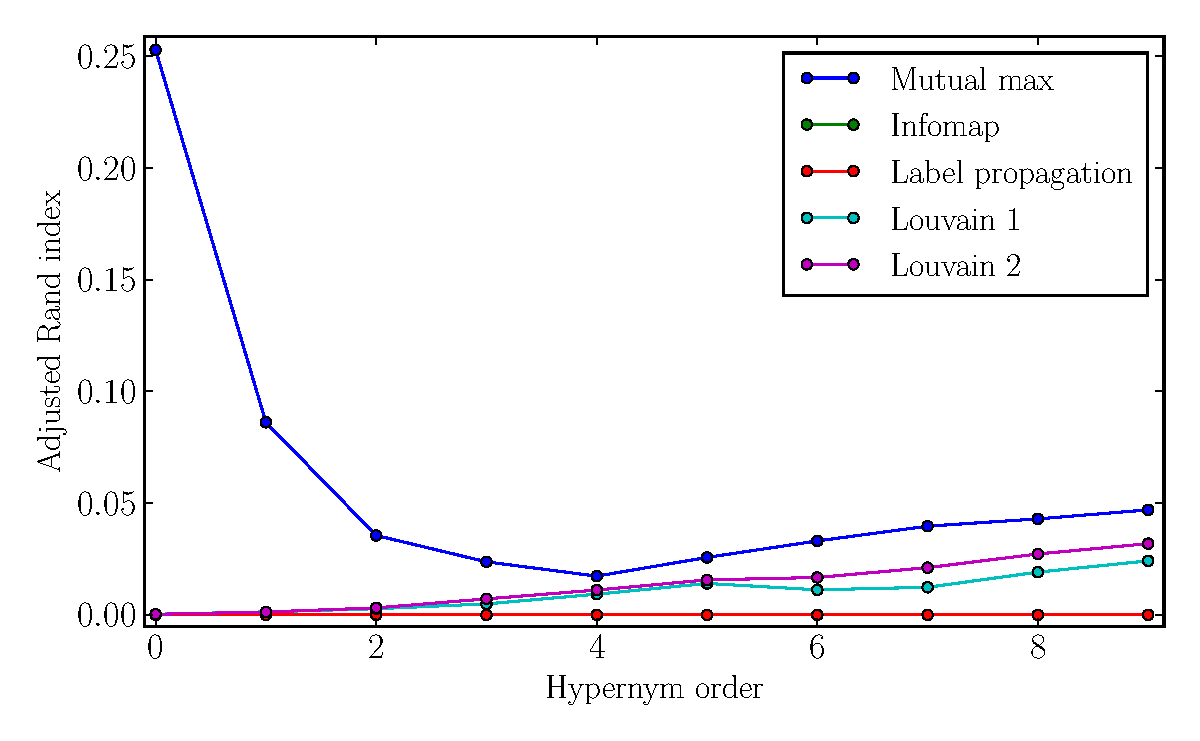
\includegraphics[width=0.9\columnwidth]{figures/1465671278-1465711376-2.pdf}
\centerline{\footnotesize{(b)}}
\end{center}
\caption{(a) Partition agreement at different levels in the word concept hierarchy with reference partitions for hypernym orders $i$.
(b) Comparison of agreements with reference partitions of words.}
\label{fig:wordplots}
\end{figure}

We now sweep the generated hierarchies while measuring agreements with the reference partitions at different levels of resolution. 

In the artist case, albeit somewhat noisy due to the relatively small dataset, the Adjusted Rand Index is 
maximized at different levels in the hierarchy for different 
reference groupings, see \fig{fig:artistplots}(a), where $ \argmax_j \ T(\pi_j, \omega_i) = 21, 20, 12, 8$ for  $i = 1, ..., 4$.
Comparing $\hat{T}(c, \omega_i)$ with the performance of the community detection algorithms (\fig{fig:artistplots}(b)) shows that our method performs
comparably well on all levels, achieving the best agreement with $\omega_i$ at three out of four levels, with
a particularly advantage for finer-grained reference groupings.

The results look very different in the word case since there are a much larger number of primitive objects (10000 instead of 500)
and many more groups in the reference partitions. In \fig{fig:wordplots}(a) we see that $T(c, \omega_i)$ has more distinct 
maxima for different hypernym orders $i$. Interestingly, there is a wide \inquotes{plateau} of intermediate 
hierarchical levels that needs to be traversed prior to reaching $\hat{T}(c, \omega_i)$ for low-resolution
partitons $\omega_i$. We can also note that the relative agreement with $\omega_i$ is higher for comparably
fine-grained and comparably coarse-grained reference partitions, relative intermediate granularity levels. 
This indicates that our method, in this setting, works better at micro and macro scales compared to at meso scales. 
One possible explanation for this is that we solely relate words through adjacency relations, that only indirectly
capture word correlations across other than very narrow windows of text.

From \fig{fig:wordplots}(b) it is evident that the community detection algorithms are not able to capture finer 
abstraction levels in the data. Although the performance of the Louvain algorithm improves for coarser target partitions, 
it is still, at all levels, significantly outperformed by our method.

\subsection{Scalability}
\label{sec: scalability}

\begin{figure}
\begin{center}
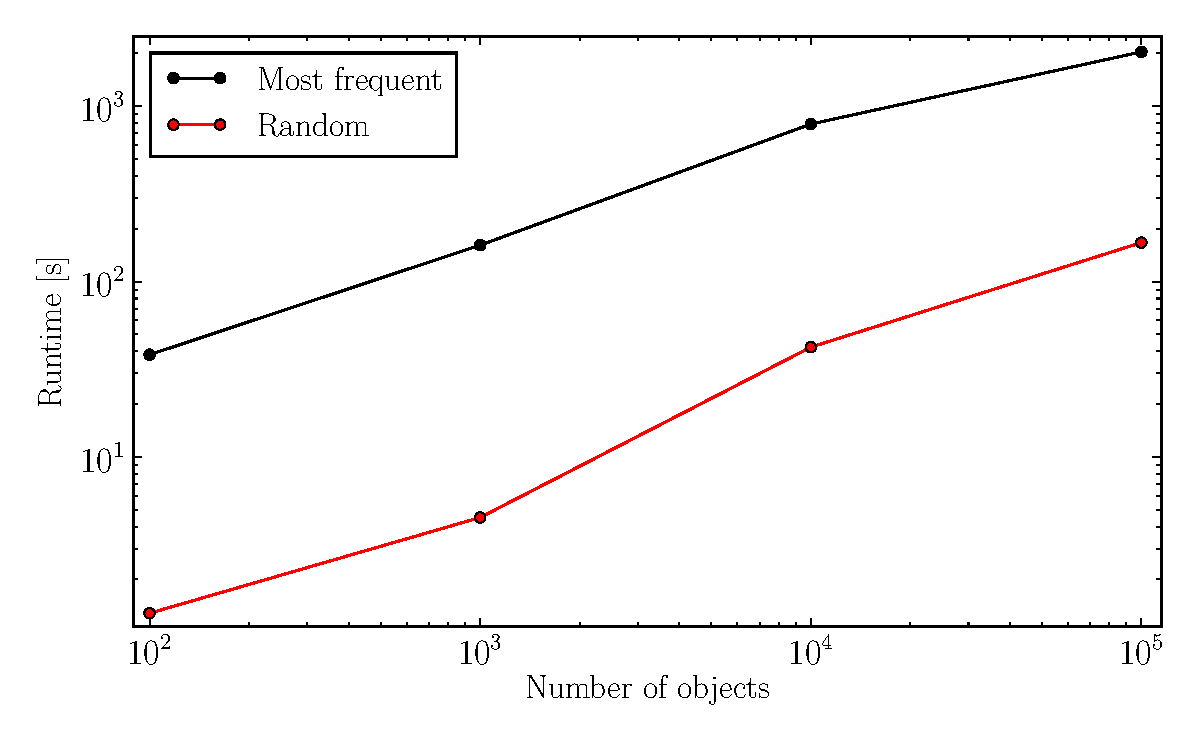
\includegraphics[width=0.9\columnwidth]{figures/wiki-runtime.pdf}
\end{center}
\caption{Runtimes for Wikipedia (10 iterations) using 24 CPUs (Intel Xeon E5-2620 v3 at 2.40GHz) and 256GB of RAM.
For different number of most frequently occurring objects and random samples of objects.}
\label{fig:runtime}
\end{figure}

Scalability is a necessary property for practical use of the method on large datasets with regard
to numbers of examples, objects and correlations.
We evaluate the scalability of the algorithm by measuring its runtime for different number of primitive objects.
Two tests are performed, both using the Wikipedia corpus, with different resulting graph densities: One where we select the most frequent words, 
and another where we use a random sample of words. In both cases the method has tractable scaling characteristics
as seen in \fig{fig:runtime}. This is due to scalable correlation to similarity graph transformations that 
utilize the sparsity of the correlation graphs \cite{Gornerup15}, combined with
efficient configuration count updates and Mutual max calculations as described in \sn{subsec:implementation}.

\section{Conclusions}
\label{sec:conclusions}
Data and generating processes can often be described on multiple abstraction levels. In this paper we have presented 
a method for discovering such levels solely using observed correlations between constituents in the data. 
We have demonstrated qualitatively and quantitatively that the method is able to conceptualize data constituents at 
multiple levels of granularity. The method uses a domain-independent and fundamental notion of similarity based on relational correlation information.
The approach is therefore not limited to a specific field, but widely applicable across domains. Furthermore, the method is parallelizable,
implemented to run in a cluster environment and scales to very large datasets. 

There are several possible improvements of the method. One shortcoming is that it does not support object polysemy.
One way to approach this is to disambiguate primitive objects prior to applying the algorithm. 
Disambiguation methods, however, are often domain-specific (see e.g.\ \cite{Cruys11}), and it would therefore be of value to incorporate disambiguation
in our domain-agnostic setting using correlation and similarity information. Another possible improvement is to enable 
overlapping concepts, which can be achieved by employing a merging criterion that does not result in disjoint groups.
These improvements are both parts of planned future work.

\section*{Acknowledgment}
\anonymize{This work was funded by the Swedish Foundation for Strategic Research (\emph{Stiftelsen f\"or strategisk forskning}) 
and the Knowledge Foundation (\emph{Stiftelsen f\"or kunskaps- och kompetensutveckling}). 
The authors would like to thank the anonymous reviewers for their valuable comments.}

% trigger a \newpage just before the given reference
% number - used to balance the columns on the last page
% adjust value as needed - may need to be readjusted if
% the document is modified later
%\IEEEtriggeratref{8}
% The "triggered" command can be changed if desired:
%\IEEEtriggercmd{\enlargethispage{-5in}}

% references section

%\newpage

\bibliographystyle{IEEEtran}
\bibliography{hierarchical-concepts}

\end{document}


